%%%%%%%%%%%%%%%%%%%%%%%%%%%%%%%%%%%%%%%%%
% Wenneker Assignment
% LaTeX Template
% Version 2.0 (12/1/2019)
%
% This template originates from:
% http://www.LaTeXTemplates.com
%
% Authors:
% Vel (vel@LaTeXTemplates.com)
% Frits Wenneker
%
% License:
% CC BY-NC-SA 3.0 (http://creativecommons.org/licenses/by-nc-sa/3.0/)
% 
%%%%%%%%%%%%%%%%%%%%%%%%%%%%%%%%%%%%%%%%%

%----------------------------------------------------------------------------------------
%	PACKAGES AND OTHER DOCUMENT CONFIGURATIONS
%----------------------------------------------------------------------------------------

\documentclass[11pt]{scrartcl} % Font size

%%%%%%%%%%%%%%%%%%%%%%%%%%%%%%%%%%%%%%%%%
% Cleese Assignment
% Structure Specification File
% Version 1.0 (27/5/2018)
%
% This template originates from:
% http://www.LaTeXTemplates.com
%
% Author:
% Vel (vel@LaTeXTemplates.com)
%
% License:
% CC BY-NC-SA 3.0 (http://creativecommons.org/licenses/by-nc-sa/3.0/)
% 
%%%%%%%%%%%%%%%%%%%%%%%%%%%%%%%%%%%%%%%%%

%----------------------------------------------------------------------------------------
%	PACKAGES AND OTHER DOCUMENT CONFIGURATIONS
%----------------------------------------------------------------------------------------

\usepackage{lastpage} % Required to determine the last page number for the footer

\usepackage{graphicx} % Required to insert images

\setlength\parindent{0pt} % Removes all indentation from paragraphs

\usepackage[most]{tcolorbox} % Required for boxes that split across pages

\usepackage{booktabs} % Required for better horizontal rules in tables

\usepackage{listings} % Required for insertion of code

\usepackage{etoolbox} % Required for if statements

%----------------------------------------------------------------------------------------
%	MARGINS
%----------------------------------------------------------------------------------------

\usepackage{geometry} % Required for adjusting page dimensions and margins

\geometry{
	paper=a4paper, % Change to letterpaper for US letter
	top=3cm, % Top margin
	bottom=3cm, % Bottom margin
	left=2.5cm, % Left margin
	right=2.5cm, % Right margin
	headheight=14pt, % Header height
	footskip=1.4cm, % Space from the bottom margin to the baseline of the footer
	headsep=1.2cm, % Space from the top margin to the baseline of the header
	%showframe, % Uncomment to show how the type block is set on the page
}

%----------------------------------------------------------------------------------------
%	FONT
%----------------------------------------------------------------------------------------

\usepackage[utf8]{inputenc} % Required for inputting international characters
\usepackage[T1]{fontenc} % Output font encoding for international characters

\usepackage[sfdefault,light]{roboto} % Use the Roboto font

%----------------------------------------------------------------------------------------
%	HEADERS AND FOOTERS
%----------------------------------------------------------------------------------------

\usepackage{fancyhdr} % Required for customising headers and footers

\pagestyle{fancy} % Enable custom headers and footers

\lhead{\small\assignmentClass\ifdef{\assignmentClassInstructor}{\ (\assignmentClassInstructor):}{}\ \assignmentTitle} % Left header; output the instructor in brackets if one was set
\chead{} % Centre header
\rhead{\small\ifdef{\assignmentAuthorName}{\assignmentAuthorName}{\ifdef{\assignmentDueDate}{Due\ \assignmentDueDate}{}}} % Right header; output the author name if one was set, otherwise the due date if that was set

\lfoot{} % Left footer
\cfoot{\small Page\ \thepage\ of\ \pageref{LastPage}} % Centre footer
\rfoot{} % Right footer

\renewcommand\headrulewidth{0.5pt} % Thickness of the header rule

%----------------------------------------------------------------------------------------
%	MODIFY SECTION STYLES
%----------------------------------------------------------------------------------------

\usepackage{titlesec} % Required for modifying sections

%------------------------------------------------
% Section

\titleformat
{\section} % Section type being modified
[block] % Shape type, can be: hang, block, display, runin, leftmargin, rightmargin, drop, wrap, frame
{\Large\bfseries} % Format of the whole section
{\assignmentQuestionName~\thesection} % Format of the section label
{6pt} % Space between the title and label
{} % Code before the label

\titlespacing{\section}{0pt}{0.5\baselineskip}{0.5\baselineskip} % Spacing around section titles, the order is: left, before and after

%------------------------------------------------
% Subsection

\titleformat
{\subsection} % Section type being modified
[block] % Shape type, can be: hang, block, display, runin, leftmargin, rightmargin, drop, wrap, frame
{\itshape} % Format of the whole section
{(\alph{subsection})} % Format of the section label
{4pt} % Space between the title and label
{} % Code before the label

\titlespacing{\subsection}{0pt}{0.5\baselineskip}{0.5\baselineskip} % Spacing around section titles, the order is: left, before and after

\renewcommand\thesubsection{(\alph{subsection})}

%----------------------------------------------------------------------------------------
%	CUSTOM QUESTION COMMANDS/ENVIRONMENTS
%----------------------------------------------------------------------------------------

% Environment to be used for each question in the assignment
\newenvironment{question}{
	\vspace{0.5\baselineskip} % Whitespace before the question
	\section{} % Blank section title (e.g. just Question 2)
	\lfoot{\small\itshape\assignmentQuestionName~\thesection~continued on next page\ldots} % Set the left footer to state the question continues on the next page, this is reset to nothing if it doesn't (below)
}{
	\lfoot{} % Reset the left footer to nothing if the current question does not continue on the next page
}

%------------------------------------------------

% Environment for subquestions, takes 1 argument - the name of the section
\newenvironment{subquestion}[1]{
	\subsection{#1}
}{
}

%------------------------------------------------

% Command to print a question sentence
\newcommand{\questiontext}[1]{
	\textbf{#1}
	\vspace{0.5\baselineskip} % Whitespace afterwards
}

%------------------------------------------------

% Command to print a box that breaks across pages with the question answer
\newcommand{\answer}[1]{
	\begin{tcolorbox}[breakable, enhanced]
		#1
	\end{tcolorbox}
}

%------------------------------------------------

% Command to print a box that breaks across pages with the space for a student to answer
\newcommand{\answerbox}[1]{
	\begin{tcolorbox}[breakable, enhanced]
		\vphantom{L}\vspace{\numexpr #1-1\relax\baselineskip} % \vphantom{L} to provide a typesetting strut with a height for the line, \numexpr to subtract user input by 1 to make it 0-based as this command is
	\end{tcolorbox}
}

%------------------------------------------------

% Command to print an assignment section title to split an assignment into major parts
\newcommand{\assignmentSection}[1]{
	{
		\centering % Centre the section title
		\vspace{2\baselineskip} % Whitespace before the entire section title
		
		\rule{0.8\textwidth}{0.5pt} % Horizontal rule
		
		\vspace{0.75\baselineskip} % Whitespace before the section title
		{\LARGE \MakeUppercase{#1}} % Section title, forced to be uppercase
		
		\rule{0.8\textwidth}{0.5pt} % Horizontal rule
		
		\vspace{\baselineskip} % Whitespace after the entire section title
	}
}

%----------------------------------------------------------------------------------------
%	TITLE PAGE
%----------------------------------------------------------------------------------------

\author{\textbf{\assignmentAuthorName}} % Set the default title page author field
\date{} % Don't use the default title page date field

\title{
	\thispagestyle{empty} % Suppress headers and footers
	\vspace{0.2\textheight} % Whitespace before the title
	\textbf{\assignmentClass:\ \assignmentTitle}\\[-4pt]
	\ifdef{\assignmentDueDate}{{\small Due\ on\ \assignmentDueDate}\\}{} % If a due date is supplied, output it
	\ifdef{\assignmentClassInstructor}{{\large \textit{\assignmentClassInstructor}}}{} % If an instructor is supplied, output it
	\vspace{0.32\textheight} % Whitespace before the author name
}
 % Include the file specifying the document structure and custom commands

%----------------------------------------------------------------------------------------
%	TITLE SECTION
%----------------------------------------------------------------------------------------

\title{	
	\normalfont\normalsize
	\textsc{University, School or Department Name}\\ % Your university, school and/or department name(s)
	\vspace{25pt} % Whitespace
	\rule{\linewidth}{0.5pt}\\ % Thin top horizontal rule
	\vspace{20pt} % Whitespace
	{\huge Assignment Title}\\ % The assignment title
	\vspace{12pt} % Whitespace
	\rule{\linewidth}{2pt}\\ % Thick bottom horizontal rule
	\vspace{12pt} % Whitespace
}

\author{\LARGE Arthur Morgan} % Your name

\date{\normalsize\today} % Today's date (\today) or a custom date

\begin{document}

\maketitle % Print the title

%----------------------------------------------------------------------------------------
%	FIGURE EXAMPLE
%----------------------------------------------------------------------------------------

\section{Image Interpretation}

\begin{figure}[h] % [h] forces the figure to be output where it is defined in the code (it suppresses floating)
	\centering
	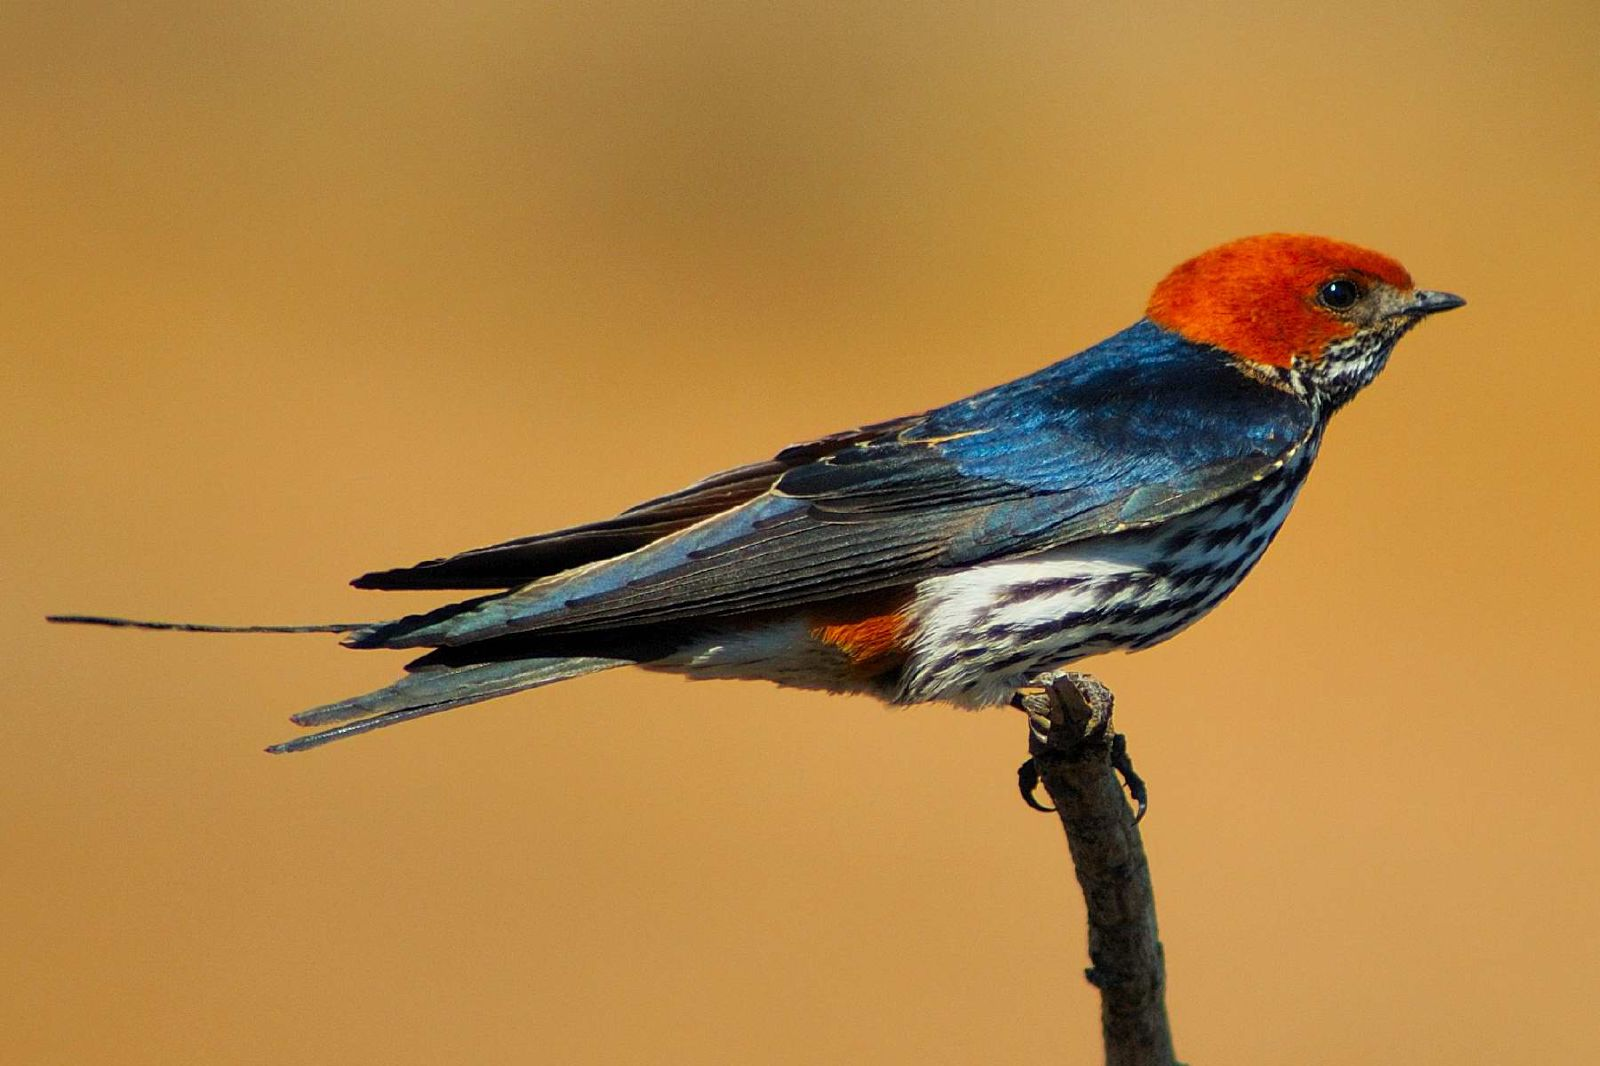
\includegraphics[width=0.5\columnwidth]{swallow.jpg} % Example image
	\caption{European swallow.}
\end{figure}

%------------------------------------------------

\subsection{What is the airspeed velocity of an unladen swallow?}

While this question leaves out the crucial element of the geographic origin of the swallow, according to Jonathan Corum, an unladen European swallow maintains a cruising airspeed velocity of \textbf{11 metres per second}, or \textbf{24 miles an hour}. The velocity of the corresponding African swallows requires further research as kinematic data is severely lacking for these species.

%----------------------------------------------------------------------------------------
%	TEXT EXAMPLE
%----------------------------------------------------------------------------------------

\section{Understanding Text}

\subsection{How much wood would a woodchuck chuck if a woodchuck could chuck wood?}

%------------------------------------------------

\subsubsection{Suppose ``chuck" implies throwing.}

According to the Associated Press (1988), a New York Fish and Wildlife technician named Richard Thomas calculated the volume of dirt in a typical 25--30 foot (7.6--9.1 m) long woodchuck burrow and had determined that if the woodchuck had moved an equivalent volume of wood, it could move ``about \textbf{700 pounds (320 kg)} on a good day, with the wind at his back".

%------------------------------------------------

\subsubsection{Suppose ``chuck" implies vomiting.}

A woodchuck can ingest 361.92 cm\textsuperscript{3} (22.09 cu in) of wood per day. Assuming immediate expulsion on ingestion with a 5\% retainment rate, a woodchuck could chuck \textbf{343.82 cm\textsuperscript{3}} of wood per day.

%------------------------------------------------

\paragraph{Bonus: suppose there is no woodchuck.}

Fusce varius orci ac magna dapibus porttitor. In tempor leo a neque bibendum sollicitudin. Nulla pretium fermentum nisi, eget sodales magna facilisis eu. Praesent aliquet nulla ut bibendum lacinia. Donec vel mauris vulputate, commodo ligula ut, egestas orci. Suspendisse commodo odio sed hendrerit lobortis. Donec finibus eros erat, vel ornare enim mattis et.

%----------------------------------------------------------------------------------------
%	EQUATION EXAMPLES
%----------------------------------------------------------------------------------------

\section{Interpreting Equations}

\subsection{Identify the author of Equation \ref{eq:bayes} below and briefly describe it in English.}

\begin{align} 
	\label{eq:bayes}
	\begin{split}
		P(A|B) = \frac{P(B|A)P(A)}{P(B)}
	\end{split}					
\end{align}

Lorem ipsum dolor sit amet, consectetur adipiscing elit. Praesent porttitor arcu luctus, imperdiet urna iaculis, mattis eros. Pellentesque iaculis odio vel nisl ullamcorper, nec faucibus ipsum molestie. Sed dictum nisl non aliquet porttitor. Etiam vulputate arcu dignissim, finibus sem et, viverra nisl. Aenean luctus congue massa, ut laoreet metus ornare in. Nunc fermentum nisi imperdiet lectus tincidunt vestibulum at ac elit. Nulla mattis nisl eu malesuada suscipit.

%------------------------------------------------

\subsection{Try to make sense of some more equations.}

\begin{align} 
	\begin{split}
		(x+y)^3 &= (x+y)^2(x+y)\\
		&=(x^2+2xy+y^2)(x+y)\\
		&=(x^3+2x^2y+xy^2) + (x^2y+2xy^2+y^3)\\
		&=x^3+3x^2y+3xy^2+y^3
	\end{split}					
\end{align}

Lorem ipsum dolor sit amet, consectetuer adipiscing elit. 
\begin{align}
	A = 
	\begin{bmatrix}
		A_{11} & A_{21} \\
		A_{21} & A_{22}
	\end{bmatrix}
\end{align}
Aenean commodo ligula eget dolor. Aenean massa. Cum sociis natoque penatibus et magnis dis parturient montes, nascetur ridiculus mus. Donec quam felis, ultricies nec, pellentesque eu, pretium quis, sem.

%----------------------------------------------------------------------------------------
%	LIST EXAMPLES
%----------------------------------------------------------------------------------------

\section{Viewing Lists}

\subsection{Bullet Point List}

\begin{itemize}
	\item First item in a list 
		\begin{itemize}
		\item First item in a list 
			\begin{itemize}
			\item First item in a list 
			\item Second item in a list 
			\end{itemize}
		\item Second item in a list 
		\end{itemize}
	\item Second item in a list 
\end{itemize}

%------------------------------------------------

\subsection{Numbered List}

\begin{enumerate}
	\item First item in a list 
	\item Second item in a list 
	\item Third item in a list
\end{enumerate}

%----------------------------------------------------------------------------------------
%	TABLE EXAMPLE
%----------------------------------------------------------------------------------------

\section{Interpreting a Table}

\begin{table}[h] % [h] forces the table to be output where it is defined in the code (it suppresses floating)
	\centering % Centre the table
	\begin{tabular}{l l l}
		\toprule
		\textit{Per 50g} & \textbf{Pork} & \textbf{Soy} \\
		\midrule
		Energy & 760kJ & 538kJ\\
		Protein & 7.0g & 9.3g\\
		Carbohydrate & 0.0g & 4.9g\\
		Fat & 16.8g & 9.1g\\
		Sodium & 0.4g & 0.4g\\
		Fibre & 0.0g & 1.4g\\
		\bottomrule
	\end{tabular}
	\caption{Sausage nutrition.}
\end{table}

%------------------------------------------------

\subsection{The table above shows the nutritional consistencies of two sausage types. Explain their relative differences given what you know about daily adult nutritional recommendations.}

Lorem ipsum dolor sit amet, consectetur adipiscing elit. Praesent porttitor arcu luctus, imperdiet urna iaculis, mattis eros. Pellentesque iaculis odio vel nisl ullamcorper, nec faucibus ipsum molestie. Sed dictum nisl non aliquet porttitor. Etiam vulputate arcu dignissim, finibus sem et, viverra nisl. Aenean luctus congue massa, ut laoreet metus ornare in. Nunc fermentum nisi imperdiet lectus tincidunt vestibulum at ac elit. Nulla mattis nisl eu malesuada suscipit.

%----------------------------------------------------------------------------------------
%	CODE LISTING EXAMPLE
%----------------------------------------------------------------------------------------

\section{Reading a Code Listing}

\lstinputlisting[
	caption=Luftballons Perl Script., % Caption above the listing
	label=lst:luftballons, % Label for referencing this listing
	language=Perl, % Use Perl functions/syntax highlighting
	frame=single, % Frame around the code listing
	showstringspaces=false, % Don't put marks in string spaces
	numbers=left, % Line numbers on left
	numberstyle=\tiny, % Line numbers styling
	]{luftballons.pl}

%------------------------------------------------

\subsection{How many luftballons will be output by the Listing \ref{lst:luftballons} above?}

Aliquam arcu turpis, ultrices sed luctus ac, vehicula id metus. Morbi eu feugiat velit, et tempus augue. Proin ac mattis tortor. Donec tincidunt, ante rhoncus luctus semper, arcu lorem lobortis justo, nec convallis ante quam quis lectus. Aenean tincidunt sodales massa, et hendrerit tellus mattis ac. Sed non pretium nibh. Donec cursus maximus luctus. Vivamus lobortis eros et massa porta porttitor.

%------------------------------------------------

\subsection{Identify the regular expression in Listing \ref{lst:luftballons} and explain how it relates to the anti-war sentiments found in the rest of the script.}

Fusce varius orci ac magna dapibus porttitor. In tempor leo a neque bibendum sollicitudin. Nulla pretium fermentum nisi, eget sodales magna facilisis eu. Praesent aliquet nulla ut bibendum lacinia. Donec vel mauris vulputate, commodo ligula ut, egestas orci. Suspendisse commodo odio sed hendrerit lobortis. Donec finibus eros erat, vel ornare enim mattis et.

%----------------------------------------------------------------------------------------

\end{document}
